%\documentclass[a4paper, 12pt]{jsbook}
%\usepackage{graphicx, booktabs, amsmath, amssymb, url, makeidx, color}
%\usepackage{sprmacros, fancybox, bm}
%\begin{document}

\section{\KLUDGE 概要}

\index{FileIO}
FileIO\KLUDGE はファイル入出力機能を提供するモジュールです.
Framework\KLUDGE から利用するのが簡単ですが、単体で用いるとより細かな作業ができます。

\section{FileIO SDK}

\index{FISdk}
FileIO\KLUDGE モジュールのすべてのオブジェクトはSDK\KLUDGE クラス\texttt{FISdk}\KLUDGE によって管理されます.
\texttt{FISdk}\KLUDGE クラスは,プログラムの実行を通してただ1つのオブジェクトが存在するシングルトンクラスです.
\texttt{FISdk}\KLUDGE オブジェクトを作成するには以下のようにします.
\begin{sourcecode}
FISdkIf* fiSdk = FISdkIf::CreateSdk();
\end{sourcecode}
\KLUDGE 通常この操作はプログラムの初期化時に一度だけ実行します.
\KLUDGE また,Framework\KLUDGE モジュールを使用する場合はユーザが直接\texttt{FISdk}\KLUDGE を作成する必要はありません.

\texttt{FISdk}\KLUDGE には以下の2\KLUDGE つの機能があります.
\begin{itemize}
\item \KLUDGE ファイルオブジェクトの作成
\item \KLUDGE インポートオブジェクトの作成
\end{itemize}

\begin{figure}[t]
\begin{center}
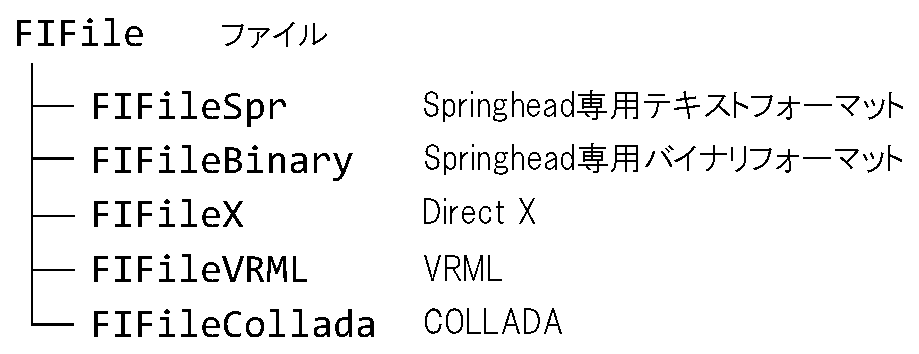
\includegraphics[width=.6\hsize]{fig/fifile.eps}
\end{center}
\caption{Class hierarchy of file objects}
\label{fig_fifile}
\end{figure}

\index{FIFile}
\index{\KLUDGE ふぁいる@\KLUDGE ファイル}
\KLUDGE ファイルオブジェクトは,ファイルからのシーンのロードおよびセーブを担います.
\KLUDGE ファイルの基底クラスは\texttt{FIFile}\KLUDGE で,ファイルフォーマットの種類ごとに専用のファイルクラスが派生します
(\Fig{fifile})\KLUDGE .

\KLUDGE ファイル作成に関する\texttt{FISdk}\KLUDGE の関数を以下に示します.

\begin{center}
\begin{tabular}{p{.3\hsize}p{.6\hsize}}
\texttt{FISdkIf}															\\ \midrule
\texttt{FIFileSprIf*}		& \texttt{CreateFileSpr()}						\\
\texttt{FIFileBinaryIf*} 	& \texttt{CreateFileBinary()}					\\
\texttt{FIFileXIf*}			& \texttt{CreateFileX()}						\\
\texttt{FIFileVRMLIf*}		& \texttt{CreateFileVRML()}						\\
\texttt{FIFileCOLLADAIf*}	& \texttt{CreateFileCOLLADA()}					\\
\texttt{FIFileIf*}			& \texttt{CreateFileFromExt(UTString filename)}	\\
\end{tabular}
\end{center}

\texttt{CreateFileFromExt}\KLUDGE は\texttt{filename}\KLUDGE の拡張子からファイルフォーマットを判別して対応するファイルオブジェクトを作成します.

\section{\KLUDGE ファイルフォーマット}
\KLUDGE この節ではSpringhead\KLUDGE でロード・セーブできるファイルのファイルフォーマットを紹介します。

\subsection{spr\KLUDGE ファイル}
\KLUDGE 拡張子 .spr \KLUDGE のファイルは、Springhead\KLUDGE 独自のファイル形式です。
\KLUDGE 人が読み書きしやすく、Springhead\KLUDGE の仕様が変化しても余り影響を受けないような形式になっています。ファイルを手書きする場合はこの形式を使ってください。

spr\KLUDGE ファイルはノード定義の繰り返しです。spr\KLUDGE ファイルの例を示します。

\begin{sourcecode}
PHSdk{                  #PHSdkノード
    CDSphere sphere{    #↑の子ノードにCDSphereノードを追加
        material = {    # CDSphere の material(PHMaterial型)の
            mu = 0.2    # 摩擦係数 mu に0.2を代入
        }
        radius = 0.5    # radiusに0.5を代入
    }
    CDBox bigBox{
        boxsize = 2.0 1.1 0.9
    }
}
\end{sourcecode}

Spr\KLUDGE ファイルのノードはディスクリプタ(\SECTION{if_desc})\KLUDGE を参照)に1対1で対応します。ディスクリプタさえ用意すれば自動的に使えるノードの型が増えます。
\KLUDGE ファイルで値を代入しないと、ディスクリプタの初期値になります。
\KLUDGE 上の例では、\texttt{PHSdk}\KLUDGE に追加される\texttt{sphere}(\texttt{CDSphere}\KLUDGE 型)\KLUDGE は、
\begin{sourcecode}
CDSphereDesc desc;
desc.material.mu = 0.2;
desc.radius = 0.5;
\end{sourcecode}
\KLUDGE としたディスクリプタ \texttt{desc} \KLUDGE で作るのと同じことになります。

Spr\KLUDGE ファイルの文法をBNF\KLUDGE +正規表現で書くと
\begin{sourcecode}
spr   = node*
node  = node type, (node id)?, block
block = '{' (node|refer|data)*  '}'
refer = '*' node id
data  = field id, '=', (block | right)
right = '[' value*, ']' | value
value = bool | int | real | str | right
\end{sourcecode}
\KLUDGE となります。\texttt{right}\KLUDGE 以降の解釈は\texttt{field}\KLUDGE の型に依存します。

\subsection{X\KLUDGE ファイル}
\KLUDGE 「 X \KLUDGE ファイル \KLUDGE 」は、Direct3D\KLUDGE のファイルフォーマットで、拡張子は .x \KLUDGE です。
\KLUDGE モデリングソフトXSI\KLUDGE で使われており、多くのモデリングツールで出力できます。
3D\KLUDGE の形状データ、マテリアル、テクスチャ、ボーンなどを含めることができます。
Springhead2\KLUDGE では、標準的なX\KLUDGE ファイルのロードと、Springhead2\KLUDGE 独自のノードの
\KLUDGE ロードとセーブができます。ただし独自ノードを手書きする場合は Spr\KLUDGE ファイル
\KLUDGE の方が書きやすく便利ですのでそちらの使用をおすすめします。

X\KLUDGE ファイルの例を示します。
\begin{sourcecode}
xof 0302txt 0064        #最初の行はこれから始まる

#    ノードは,
#        型名,ノード名 { フィールドの繰り返し   子ノード }
#    からなる.
PHScene scene1{
    0.01;0;;            #フィールド は 値; の繰り返し
    1;0;-9.8;0;;        #値は 数値,文字列またはフィールド
    PHSolid soFloor{    #子ノードは,ノードと同じ
        (省略)
    }
}
# コメントは #以外に // も使える
\end{sourcecode}

\subsubsection{\KLUDGE 独自ノードの定義}
Springhead2 \KLUDGE の通常のノードは,オブジェクトのディスクリプタ(\SECTION{if_desc}\KLUDGE 節)に1対1で対応します.
\KLUDGE ロード時には,ディスクリプタに対応するオブジェクトが生成され,シーングラフに追加されます.
\KLUDGE セーブ時には,オブジェクトからディスクリプタを読み出し,ノードの形式でファイルに保存されます.

\KLUDGE オブジェクトのディスクリプタには,必ず対応するノードがあります.
\KLUDGE 例えば,\texttt{SprPHScene.h} \KLUDGE には,

\begin{sourcecode}
struct PHSceneState{
    double timeStep;      ///< 積分ステップ
    unsigned count;       ///< 積分した回数
};
struct PHSceneDesc:PHSceneState{
    /// 接触・拘束解決エンジンの種類
    enum ContactMode{ MODE_NONE, MODE_PENALTY, MODE_LCP};
    Vec3f gravity;      ///< 重力加速度ベクトル.デフォルト値は(0.0f, -9.8f,0.0f).
};
\end{sourcecode}

\KLUDGE のように,ステートとディスクリプタが宣言されています.この \texttt{PHSceneDesc} \KLUDGE に対応する X \KLUDGE ファイルのノードは,
\begin{sourcecode}
PHScene scene1{                                                                     0.01;     #PHSceneState::timeStep
    0;;       #PHSceneState::count     最後の;はPHSceneState部の終わりを示す.
    1;        #PHSceneDesc::ContactMode
    0;-9.8;0;;#PHSceneDesc::gravity    最後の;はPHSceneDesc部の終わりを示す.
}
\end{sourcecode}

\KLUDGE のようになります.クラスのメンバ変数がそのままフィールドになります.
\KLUDGE また,基本クラスは,先頭にフィールドが追加された形になります.

\KLUDGE 通常ノードの一覧は \URL{TBU: \KLUDGE デスクリプタ一覧のページ} \KLUDGE を参照下さい.

\subsubsection{X\KLUDGE ファイルのノード}
Springhead2\KLUDGE の独自ノードだけでなく、普通のX\KLUDGE ファイルのノードもロードできます。
X\KLUDGE ファイルには、
\begin{sourcecode}
Frame{
    FrameTransfromMatrix{ 1,0,0,0, 0,1,0,0, 0,0,1,0, 0,0,0,1; }
}
\end{sourcecode}
\KLUDGE のようなフレームのノード型がありますが、
Sprinhead2 \KLUDGE には対応するディスクリプタやオブジェクトがありません.
\KLUDGE そこで,これらは、\texttt{GRFrame}\KLUDGE や\texttt{PHFrame}\KLUDGE に
\KLUDGE 変換されてロードされます.
\URL{TBW \KLUDGE ノード一覧のページ(pageNodeDefList)} \KLUDGE を参照下さい.


\section{\KLUDGE ファイルのロード・セーブ}
\begin{figure}
\begin{center}
\includegraphics*[width=.95\hsize]{fig/fileOperation.eps}
\end{center}
\caption{Overview of file operation}
\label{fig_fileOperation}
\end{figure}

\Fig{fileOperation}\KLUDGE は、ファイルのロード・セーブの手順を示しています。
\KLUDGE ロード時にはまずファイルをパースしてディスクリプタのツリーを作ります。
\KLUDGE 次にディスクリプタのツリーをたどりながら、オブジェクトのツリーを作ります。
\KLUDGE 一方、セーブ時には、ディスクリプタツリーは作りません。
\KLUDGE オブジェクトツリーをたどりながらオブジェクトからディスクリプタを作り、その場でファイルに書きだしていきます。

\KLUDGE ファイルのノードとディスクリプタツリーのノードは1対1に対応しますが、オブジェクトのツリーではそうとは限りません。

\subsection{\KLUDGE ファイルロードの仕組み}
\subsubsection{\KLUDGE ファイルのパース}
\KLUDGE ファイルのロードは、\texttt{FIFileSpr}\KLUDGE や\texttt{FIFileX}\KLUDGE のような\texttt{FIFile}\KLUDGE の派生クラスの\texttt{LoadImp()}\KLUDGE メソッドが行います。
\KLUDGE ファイルパースの実装は、boost::spirit\KLUDGE を用いて実装されています。\texttt{Init()}\KLUDGE メソッドでパーサの文法を定義しています。
\subsubsection{\KLUDGE ディスクリプタの生成}
\KLUDGE パーサは\texttt{FILoadContext}\KLUDGE をコンテキストとして用いながらパースを進めます。
\texttt{fieldIts}\KLUDGE にロード中のデータの型情報をセットしていきます。
\KLUDGE ノード名やメンバ名からディスクリプタやメンバの型を知る必要がありますが、ビルド時にSWIG\KLUDGE で生成しているディスクリプタの型情報を\texttt{??Sdk::RegisterSdk()}\KLUDGE が登録したものを用いています。
\KLUDGE 新しいノードが出てくる度に\texttt{FILoadContext::datas}\KLUDGE にディスクリプタを用意し、データをロードするとそこに値をセットしていきます。
\KLUDGE 他のノードへの参照は、この時点ではノード名の文字列で記録しておきます。
\subsubsection{\KLUDGE 参照のリンク}
\KLUDGE ファイルをすべてロードし終わると、\texttt{LoadImp()}\KLUDGE から抜けて、\texttt{FIFile::Load(FILoadContext*)}\KLUDGE に戻ってきます。
\KLUDGE 他のノード(\KLUDGE 他のディスクリプタ)\KLUDGE への参照をノード名の文字列を頼りにポインタでつないでいきます。
\subsubsection{\KLUDGE オブジェクトの生成}
\KLUDGE オブジェクト生成は、\texttt{FILoadContext::CreateScene()}\KLUDGE が、
\KLUDGE ディスクリプタツリーを根本からたどりながら順に行います。
\KLUDGE ディスクリプタからオブジェクトを生成するのは、そのオブジェクトの先祖オブジェクトです。先祖オブジェクトが生成できない場合はSDK\KLUDGE の生成を試みます。
SDK\KLUDGE 以外が一番根本にあるファイルをロードするためには、予め先祖オブジェクトを用意しておく必要があります。
\texttt{FIFile::Load(ObjectIfs\& objs, const char* fn)}\KLUDGE の\texttt{objs}\KLUDGE 引数はその役割をします。

\KLUDGE 生成されたオブジェクトは、親の\texttt{AddChildObject()}\KLUDGE ですぐに子として追加されます。

\subsubsection{\KLUDGE 参照のリンク}
\KLUDGE ディスクリプタ間の参照はポインタになっていますが、シーングラフは繋がっていません。ディスクリプタの参照に従って、ディスクリプタから生成されたオブジェクト間に参照を追加します。リンクは、\texttt{AddChildObject()}\KLUDGE 関数を呼び出すことで行われます。親子と参照の区別はつかなくなります。あるノードの下に子ノードを書いても、別のところに書いたノードへの参照を書いても同じシーグラフになるわけです。

\subsection{\KLUDGE ファイルロードの実際}
Framework\KLUDGE を使うのと簡単です。
\begin{sourcecode}
virtual void FWMyApp::Init(int argc, char* argv[]){
    UTRef<ImportIf> import = GetSdk()->GetFISdk()->CreateImport();
    GetSdk()->LoadScene(fileName, import);  // ファイルのロード
    GetSdk()->SaveScene("save.spr", import);// ファイルのセーブテスト
\end{sourcecode}

FISdk\KLUDGE 単体で使う場合は次のようになります。
\begin{sourcecode}
int main(){
    //  ファイルローダで生成できるように、各SDKの型情報を登録
    PHSdkIf::RegisterSdk();
    GRSdkIf::RegisterSdk();
    FWSdkIf::RegisterSdk();
    //  ファイルのロード
    UTRef<FISdkIf> fiSdk = FISdkIf::CreateSdk();
    FIFileIf* file = fiSdk->CreateFileFromExt(".spr");
    ObjectIfs objs; //  ロード用オブジェクトスタック
    fwSdk = FWSdkIf::CreateSdk();   //  FWSDKを用意
    //  子オブジェクト作成用にfwSdkをスタックに積む
    objs.push_back(fwSdk);
    //  FWSDK以下全体をファイルからロード
    if (! file->Load(objs, "test.spr") ) {  
        DSTR << "Error: Cannot open load file. " << std::endl;
        exit(-1);
    }
    //  ファイル中のルートノード(複数の可能性あり)がobjsに積まれる。
    for(unsigned  i=0; i<objs.size(); ++i){ 
        objs[i]->Print(DSTR);
    }
    ...
\end{sourcecode}

\subsection{\KLUDGE ファイルセーブの仕組み}
\KLUDGE ファイルセーブは、\texttt{FIFile}\KLUDGE がシーングラフをたどりながら、オブジェクトをセーブしていきます。
\KLUDGE 各オブジェクトの
\texttt{GetDescAddress()}\KLUDGE か、実装されていなければ\texttt{GetDesc()}\KLUDGE を呼び出して
\KLUDGE ディスクリプタを読み出します。
\KLUDGE シーングラフには、あるノードが複数のノードの子ノードになっている場合があるため、2\KLUDGE 重にセーブしないように2\KLUDGE 度目以降は参照としてセーブします。

\KLUDGE ディスクリプタを取り出したら、ディスクリプタの型情報を利用して、ディスクリプタのメンバを順番にセーブしていきます。
\KLUDGE 実際にデータをファイルに保存するコードは、\texttt{FiFileSpr}\KLUDGE など\texttt{FiFile}\KLUDGE の派生クラスにあります。

\subsection{\KLUDGE ファイルセーブの実際}
Framework\KLUDGE を使うのと簡単です。
\begin{sourcecode}
virtual void FWMyApp::Save(const char* filename){
    UTRef<ImportIf> import = GetSdk()->GetFISdk()->CreateImport();
    GetSdk()->SaveScene(filename, import);	// filenameにシーンをセーブ
\end{sourcecode}

FISdk\KLUDGE 単体で使う場合は次のようになります。
\begin{sourcecode}
void save(const char* filename, ImportIf* ex, ObjectIf* rootNode){
    //  ファイルのセーブ
    UTRef<FISdkIf> fiSdk = FISdkIf::CreateSdk();
    FIFileIf* file = fiSdk->CreateFileFromExt(".spr");
    ObjectIfs objs; //  ロード用オブジェクトスタック
    objs.push_back(rootNode);
    file->SetImport(ex);
    file->Save(*objs, filename);
}
\end{sourcecode}

\section{\KLUDGE インポート情報の管理}
T.B.W.
\KLUDGE (Import\KLUDGE を使うと別のファイルに書いたノードを呼び出すことができる。
Import\KLUDGE を使ってロードしたシーンをセーブ場合、ファイル保存時にどこまでを
\KLUDGE ファイルに保存するのかが問題になる。
\KLUDGE これを管理するのがImport\KLUDGE の役割だと思う。by \KLUDGE 長谷川)
%\end{document}
